Una vez que entendemos el simulador y usamos el graficador con un scheduler básico como lo es SchedFCFS nos proponemos a realizar nuevos schedulers: \textbf{SchedRR} y \textbf{SchedLottery}.

\subsection{SchedRR}

El siguiente paso fue completar la implementación de SchedRR, el cual se basa en el algoritmo de scheduling $round-robin$. 

Básicamente las tareas forman una ronda para correr en algún núcleo (de haber más de uno). Cada CPU tiene asociado un quantum máximo, es decir, una cantidad máxima de ciclos en el cual puede correr una determinada tarea. El quantum de cada CPU es parámetro de nuestro scheduler.

Así como el SchedFCFS, éste scheduler esta implementado sobre una cola de tareas global (para permitir migración), pero a diferencia del anterior, nuestro scheduler irá encolando a las tareas nuevamente en la cola una vez que sean desalojadas del CPU, ya sea por realizar una llamada bloqueante o debido a que su quantum se completó. Si la tarea se bloqueo, no sera encolada en la cola de tareas $ready$ hasta que se desbloquee, por lo cual la función UNBLOCK comienza a tener sentido y es ahi donde la tarea regresa a la cola.

Para determinar si una tarea cumplió con el quantum máximo del CPU en la cual corre tenemos un vector de quantums parciales, un contador para cada CPU. Por cada tick se incrementa en uno y se resetea en caso de que la tarea sea desalojada. Notar que si la tarea se bloquea es desalojada y por lo tanto pierde su quantum.

Como detalle de implementación determinamos que si alguna tarea se bloquea y no hay ninguna tarea lista para correr, es decir, la cola de tareas $ready$ esta vacia, ésta seguirá corriendo en el CPU para evitar pagar costos de cambio de contexto.

Veamos el gráfico a continuación:

\begin{figure}[H]
\centering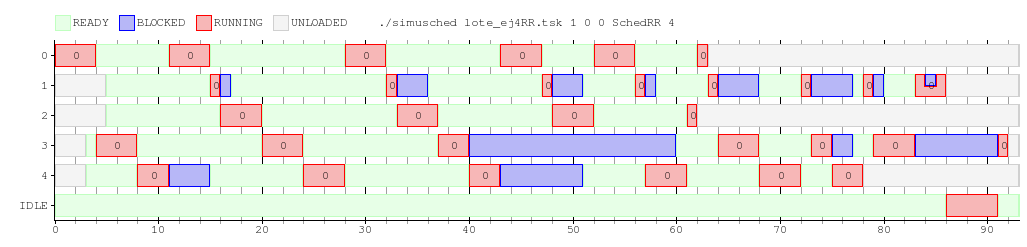
\includegraphics[width=15 cm]{graficos/ej4RR1.png}
\centering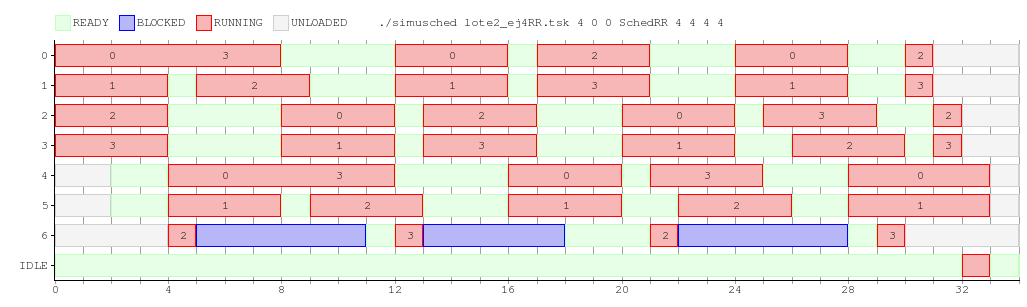
\includegraphics[width=15 cm]{graficos/ej4RR2.png}
\caption{Round-robin, un sólo núcleo de procesamiento en el primer caso, 4 en el segundo. Distintos lotes de tareas.}
\end{figure}

Se confeccionaron dos lotes diferentes para la figura 2. Para el primer caso se corrieron dos TaskCPU, una TaskConsola y dos TaskAlterno (alternan entre uso de CPU y llamadas bloqueantes). Como el primer gráfico muestra el comportamiento con un único núcleo es facil ver como SchedRR funciona. En orden de llegada cada tarea corre su quantum, o lo pierde si se bloquea para que otra tome su lugar.

El segundo caso refleja el mismo funcionamiento pero quad-core, con iguales quantums máximos para cada CPU. En este caso el lote estaba compuesto por seis TaskCPU y sólo una TaskConsola. Como en el ejemplo no hay costos de migración, algunas tareas terminan el quantum de un núcleo y automáticamente corren en otro, pero es de esperarse. La TaskConsola se bloquea y libera el CPU para otras tareas.

\subsection{SchedLottery y compensaciones probabilísticas}

\subsubsection{Ecuanimidad del SchedLottery}

En el ejercicio 5 implementamos un scheduler en base al paper ''Lottery scheduling''. Intentamos generar un mecanismo de control eficiente, flexible y justo en donde cada tarea fuese procesada
aproximadamente un tiempo equivalente a las otras, sin importar su tipo. Este último aspecto es el que nos permite hablar de ecuanimidad del scheduler.

Para ejemplificar lo mencionado anteriormente, supongamos que en una computadora de un solo core se han lanzado dos procesos que corren en simultáneo. El primero de ellos, al cual llamaremos $A$, utiliza
activamente el CPU sin necesidad de hacer llamados al sistema o esperar que se liberen recursos de la máquina (podría ser, por ejemplo, el caso de una aplicación científica que ejecuta gran cantidad de 
cuentas). Por otro lado tenemos a la tarea $B$, que ejecuta una instrucción bloqueante cada cierto tiempo, desbloquéandose luego de una cierta cantidad de ticks del reloj. Supongamos también que ambos conviven
con otros procesos que también están siendo ejecutados por el cpu. En el caso de un scheduler Round Robin, a lo largo de una ronda se le asigna un quantum a cada proceso. Sin embargo, notemos que mientras
la tarea $A$ utiliza la totalidad del quantum que le han asignado, $B$ usa únicamente una fracción: $\frac{f}{q}$. De esta manera, luego de sucesivas rondas la tarea $A$ ha sido ejecutada un tiempo
considerablemente mayor al de $B$.

Para solucionar este problema, la idea es que el scheduler seleccione la próxima a ser ejecutada mediante el sorteo de una lotería, en donde aquellas tareas que utilicen solamente una fracción del quantum
tengan más probabilidades de ser las ganadoras. Para lograr este objetivo, utilizamos un sistema de ''compensation tickets'', que funciona de la siguiente manera:

- Las tareas que llegan por primera vez entran con una cantidad equivalente a $\frac{tickets}{1 \ quantum}$. Por ejemplo, si el 
- Las tareas que utilizaron la totalidad del quantum la último





 

